\documentclass{article}

\usepackage[utf8]{inputenc}
\usepackage{amsmath, amssymb}
\usepackage{enumitem}
\usepackage{pdfpages}


\title{CS3SD3 - Assignment 3}
\author{Hien Tu - tun1}


\begin{document}

\maketitle

\section*{Question 1}

The colour petri net is at the end of the file. \\
The invariants of the petri net are:
\begin{enumerate}
  \item[(i1)] M($\text{p}_1$) + M($\text{p}_2$) + M($\text{p}_3$) +
              M($\text{p}_4$) + M($\text{p}_5$) = ph1 + ph2 + ph3 + ph4 + ph5
  \item[(i2)] LEFT(M($\text{p}_3$)) + LEFT(M($\text{p}_4$)) +
              RIGHT(M($\text{p}_4$)) + RIGHT(M($\text{p}_5$)) + M($\text{p}_6$)
              = $\text{f}_1$ + $\text{f}_2$ + $\text{f}_3$ + $\text{f}_4$ +
              $\text{f}_5$ \\
              where LEFT($X$) = $\sum_{x \in X} \text{LEFT}(x)$ and
                    RIGHT($X$) = $\sum_{x \in X} \text{RIGHT}(x)$
\end{enumerate}
If M($\text{p}_4$) $\neq \emptyset$, i.e., ph$j$ $\in$ M($\text{p}_4$), then
(return\_left\_fork, x = ph$j$) can be fired. \\
If M($\text{p}_5$) $\neq \emptyset$, i.e., ph$j$ $\in$ M($\text{p}_5$), then
(return\_right\_fork\_and\_exit\_dining\_room, x = ph$j$) can be fired. \\
If M($\text{p}_4$) $= \emptyset$ and M($\text{p}_5$) $= \emptyset$
\begin{itemize}
  \item If M($\text{p}_3$) $\neq \emptyset$
        \begin{itemize}
          \item Since we only have 4 tokens $t$, we know that only at most 4
                philosophers (ph) can reach $\text{p}_2$ and $\text{p}_3$
          \item Thus, only at most 4 forks (f) are not in $\text{p}_6$
          \item This means there is at least 1 fork in $\text{p}_6$
          \item So M($\text{p}_6$) $\neq \emptyset$
          \item Since M($\text{p}_3$) $\neq \emptyset$ and M($\text{p}_6$) $\neq
                \emptyset$, (take\_right\_fork, x = ph$i$) where ph$i$ $\in$ PH,
                can be fired.
        \end{itemize}
  \item If M($\text{p}_3$) $= \emptyset$
        \begin{itemize}
          \item If M($\text{p}_2$) $\neq \emptyset$
                \begin{itemize}
                  \item Since M($\text{p}_3$) $= \emptyset$, M($\text{p}_4$) $=
                        \emptyset$ and M($\text{p}_5$) $= \emptyset$, from (i2),
                        we know that M($\text{p}_6$) = $\text{f}_1$ +
                        $\text{f}_2$ + $\text{f}_3$ + $\text{f}_4$ +
                        $\text{f}_5$
                  \item This means M($\text{p}_6$) $\neq \emptyset$
                  \item Since M($\text{p}_2$) $\neq \emptyset$ and
                        M($\text{p}_6$) $\neq \emptyset$, (take\_left\_fork, x =
                        ph$i$) where ph$i$ $\in$ PH, can be fired
                \end{itemize}
          \item If M($\text{p}_2$) $= \emptyset$
                \begin{itemize}
                  \item Then we know M($\text{p}_2$) $= \emptyset$,
                        M($\text{p}_3$) $= \emptyset$, M($\text{p}_4$) $=
                        \emptyset$, M($\text{p}_5$) $= \emptyset$
                  \item Thus, from (i1), we have M($\text{p}_1$) = ph1 + ph2 +
                        ph3 + ph4 + ph5 and M($\text{p}_7$) $\neq \emptyset$
                  \item This case happens right at the start of the process (at
                        the initial marking) and so, (enter\_dining\_room, x =
                        ph$i$) where ph$i$ $\in$ PH, can be fired.
                \end{itemize}
        \end{itemize}
\end{itemize}
Therefore, in any case, at least one state will be able to fire.

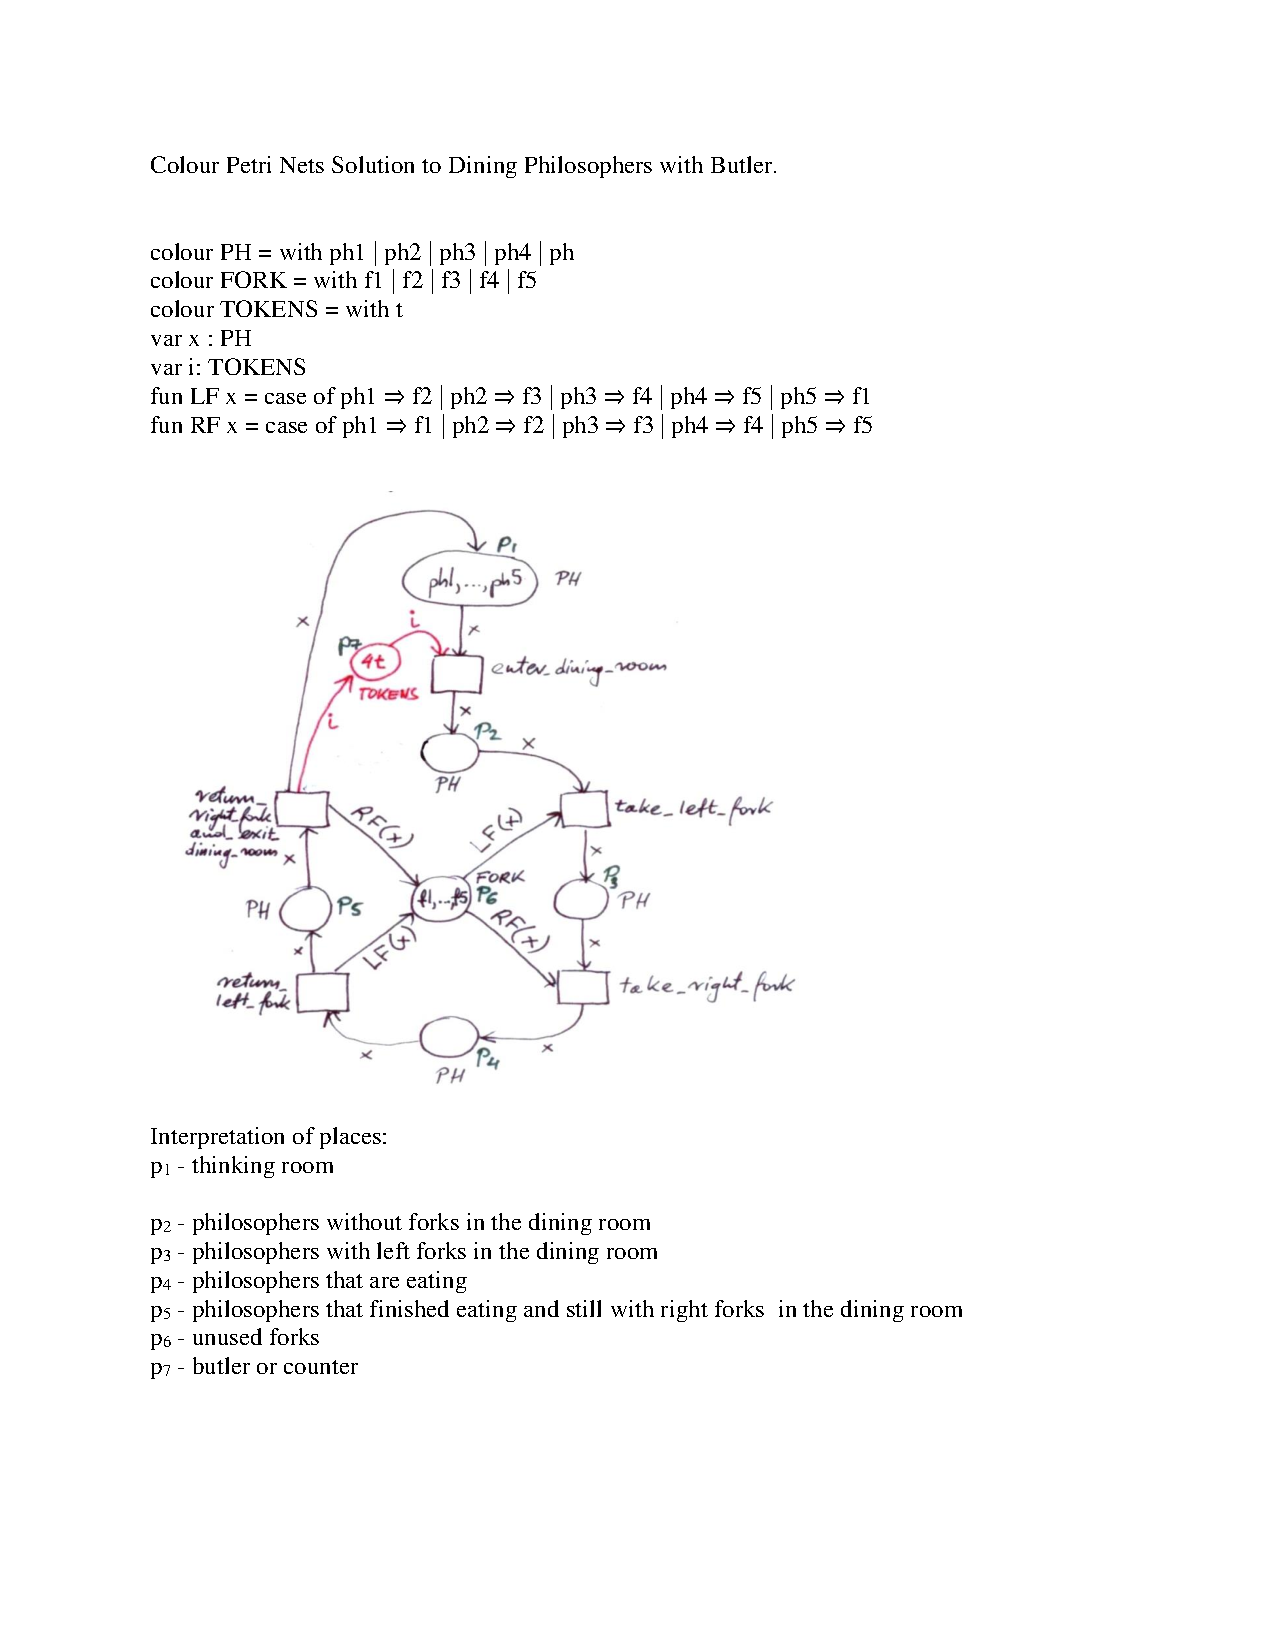
\includepdf{CPN-Butler[4427].pdf}

\end{document}